\chapter*{Приложение Б. Результаты выполнения программы}
\label{sec:appendix_problems}
\section*{Мир Лампы}

\subsection*{Описание на языке DOT}

\begin{verbatim}
digraph G {
  1 [ label="(-S -L B)" ];
  2 [ label="(S L B)" ];
  3 [ label="(S L? B?)" ];
  4 [ label="(S -L -B)" ];
  5 [ label="(S? -L B?)" ];
  6 [ label="(-S -L B?)" ];
  7 [ label="(S? -L -B)" ];
  8 [ label="(-S -L -B)" ];
  1 -> 2 [ label="on_light" ];
  3 -> 4 [ label="~B" ];
  5 -> 4 [ label="S" ];
  5 -> 1 [ label="B" ];
  5 -> 3 [ label="on_light" ];
  3 -> 2 [ label="B" ];
  5 -> 6 [ label="off_light" ];
  6 -> 1 [ label="ch_bulb" ];
  5 -> 6 [ label="~S" ];
  5 -> 7 [ label="~B" ];
  7 -> 8 [ label="off_light" ];
  7 -> 4 [ label="S" ];
  8 -> 1 [ label="ch_bulb" ];
  7 -> 8 [ label="~S" ];
  3 -> 2 [ label="L" ];
  6 -> 1 [ label="B" ];
  6 -> 3 [ label="on_light" ];
  6 -> 8 [ label="~B" ];
  3 -> 4 [ label="~L" ];
  4 -> 8 [ label="off_light" ];
  3 -> 6 [ label="off_light" ];
}
\end{verbatim}

\subsection*{Изображение графа}

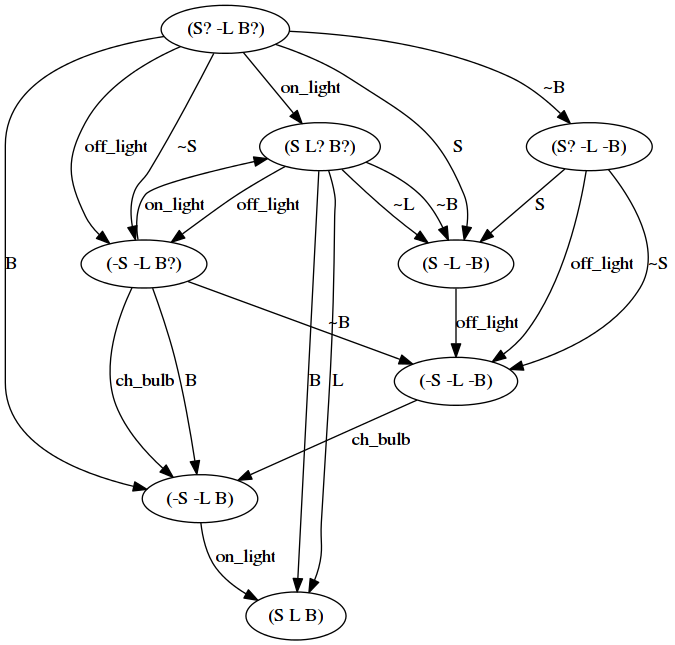
\includegraphics[width=1.0\textwidth]{plan.png}

\begin{comment}
\section*{Мир Сигнализации}

\subsection*{Описание на языке DOT}

\subsection*{Изображение графа}
\end{comment}